% ==============================================================================
% intro_stata_session.tex -- deck for the 2-hour Intro to Stata session
% Intro to Stata session, University of Groningen, Fri 11 Sep 2026
% Theme: "The Prompt" -- every frame title begins with Stata's maroon `. `
% Role : scaffolding. Front matter + segment dividers. Stata itself is the show.
% ==============================================================================
\documentclass[aspectratio=169,11pt]{beamer}

\usetheme{default}
\usecolortheme{default}
\usefonttheme{professionalfonts}
\setbeamertemplate{navigation symbols}{}

\usepackage[T1]{fontenc}
\usepackage{lmodern}               % keeps LM Typewriter as the mono face
\usepackage[sfdefault]{roboto}     % body sans
\usepackage{tikz}
\usetikzlibrary{arrows.meta, positioning}
\usepackage{graphicx}
\usepackage{ragged2e}
\usepackage{array}

% ---------- palette: "The Prompt" --------------------------------------------
\definecolor{PromptMaroon}{HTML}{8C2F39}  % core accent: the prompt
\definecolor{SlateTeal}{HTML}{3E6B74}     % secondary accent
\definecolor{Ink}{HTML}{22303F}           % body text / divider ground
\definecolor{WarmGray}{HTML}{6B6560}      % captions on Paper (5.4:1)
\definecolor{MutedOnInk}{HTML}{9AA5B1}    % captions on Ink (5.4:1) -- WarmGray
                                          % on Ink is only 2.34:1, never use it
\definecolor{Paper}{HTML}{FAF8F3}         % slide ground
\definecolor{PaperDark}{HTML}{EFE9DE}     % box fill on Paper
\definecolor{PaperSoft}{HTML}{ECE7DC}     % light mono text on Ink
\definecolor{Amber}{HTML}{C98A2D}         % prompt + emphasis on dark grounds
\definecolor{SoftBlue}{HTML}{7A9CC6}      % mono inventories on dark grounds
\definecolor{Forest}{HTML}{2F6B4F}        % "passed"
\definecolor{Alert}{HTML}{A6552E}         % the gotcha

\setbeamercolor{background canvas}{bg=Paper}
\setbeamercolor{normal text}{fg=Ink}
\setbeamercolor{frametitle}{fg=Ink}
\setbeamerfont{frametitle}{series=\bfseries,size=\Large}

% frame title = the prompt motif
\setbeamertemplate{frametitle}{%
  \vspace*{0.55cm}%
  {\ttfamily\bfseries\color{PromptMaroon}.\hspace{0.45em}}%
  {\usebeamerfont{frametitle}\usebeamercolor[fg]{frametitle}\insertframetitle}%
}

% quiet slide number, bottom right
\setbeamertemplate{footline}{%
  \hfill{\color{WarmGray}\scriptsize\insertframenumber}\hspace*{3mm}\vspace*{2mm}%
}

% ---------- TikZ styles (all in the preamble; none inside frames) ------------
\tikzset{
  win/.style={draw=WarmGray, thick, fill=PaperDark, align=center,
              inner sep=0pt},
  winlab/.style={font=\ttfamily\bfseries, text=Ink},
  windesc/.style={font=\scriptsize, text=WarmGray},
  flowbox/.style={draw=Ink, thick, fill=PaperDark, align=center,
                  minimum width=3.8cm, minimum height=2.2cm, inner sep=2pt},
  statabox/.style={draw=PromptMaroon, very thick, fill=PromptMaroon!12!Paper,
                   align=center, minimum width=2.2cm, minimum height=2.2cm},
  flowarrow/.style={-{Stealth[length=3mm]}, very thick, draw=Ink},
  tl/.style={draw=WarmGray, thin, align=center, minimum height=1.0cm,
             inner sep=0pt, fill=PaperDark, text=Ink, font=\small},
  tlpay/.style={draw=PromptMaroon, thin, align=center, minimum height=1.0cm,
                inner sep=0pt, fill=PromptMaroon, text=white,
                font=\small\bfseries},
  tlmin/.style={font=\scriptsize, text=WarmGray},
  tla/.style={draw=WarmGray, dashed, thin, align=center, minimum height=1.0cm,
              inner sep=1pt, fill=Paper, text=Ink, font=\small},
  tlbreak/.style={draw=WarmGray, dashed, thin, minimum height=1.0cm,
                  inner sep=0pt, fill=Paper},
  rowlab/.style={font=\scriptsize\itshape, anchor=east},
}

% ---------- repo-map tag chips -----------------------------------------------
% Fixed-width leading chips so the mono paths align in one column.
\newcommand{\tagtoday}{\makebox[2.5cm][l]{\colorbox{PromptMaroon}{%
  \color{white}\scriptsize\strut together, today}}}
\newcommand{\tagown}{\makebox[2.5cm][l]{\fcolorbox{WarmGray}{Paper}{%
  \color{WarmGray}\scriptsize\strut on your own}}}

% ---------- divider macro ----------------------------------------------------
% \divider{segment no.}{assertion title}{mono inventory line(s)}{minutes}
\newcommand{\divider}[4]{%
{\setbeamercolor{background canvas}{bg=Ink}%
\begin{frame}[plain]
  \centering
  \vfill
  {\ttfamily\bfseries\color{Amber}\Large .\hspace{0.45em}}%
  {\ttfamily\color{PaperSoft}segment #1}\\[1.1em]
  {\color{white}\huge\bfseries #2}\\[1.6em]
  {\ttfamily\color{SoftBlue}#3}\\[0.9em]
  {\color{MutedOnInk}\small #4 minutes}
  \vfill
\end{frame}}}

\begin{document}

% ============================================================== 1 -- title ===
{\setbeamercolor{background canvas}{bg=Ink}%
\begin{frame}[plain]
  \centering
  \vfill
  {\ttfamily\bfseries\color{Amber}\Large .\hspace{0.45em}}%
  {\color{white}\Huge\bfseries Intro to Stata}\\[1.0em]
  {\color{PaperSoft}\large A two-hour hands-on session}\\[0.35em]
  {\color{MutedOnInk}University of Groningen}\\[2.2em]
  {\color{PaperSoft}Ade Febriady}\\[0.35em]
  {\color{MutedOnInk}\small Friday 11 September 2026 \,\textperiodcentered\,
   11:00--13:00}\\[2.0em]
  {\ttfamily\color{SoftBlue}\large github.com/febriady/intro-to-stata}
  \vfill
\end{frame}}

% =============================================================== 2 -- hook ===
% The hook is a two-beat story, not a bare number. Slide 2 asks the question
% every student in the room has money on; slide 3 lands the data's insulting
% answer and names the tension (worthless education, or wrong data). The
% session is the investigation that finds the errors -- say ERROR, not lie:
% fifteen values are typos, not deception, and the lesson is "data contain
% mistakes; look before you believe". Segment 2 runs
% -correlate hwage schooling- live and prints this exact number, so the
% deck's promise and the room's experience are the same object.
\begin{frame}{Does a year of school raise your wage?}
  \vfill
  \centering
  {\Large 8{,}000 simulated wage workers}\\[0.9em]
  {\color{WarmGray}shaped on a real Indonesian survey from 2014, the one
   behind the paper\\ you will meet at the end. today you put the question
   to the data yourself}
  \vfill
  \raggedleft
  {\small\color{WarmGray}\itshape (you are betting a degree's worth of
   tuition that the answer is yes)}
  \par\vspace*{0.3cm}
\end{frame}

% ========================================================= 3 -- the answer ===
\begin{frame}{Stata's first answer: no}
  \vfill
  \centering
  {\ttfamily\bfseries\color{PromptMaroon}\fontsize{66}{70}\selectfont -0.0003}\\[1.6em]
  {\color{WarmGray}corr(wage, schooling), the laziest question you can
   ask these data}
  \vfill
  \raggedleft
  {\small\color{PromptMaroon}\itshape the data contain ordinary errors;
   the mistake is computing before looking.\\ by 13:00 you will have
   looked, and answered the question properly}
  \par\vspace*{0.3cm}
\end{frame}

% ============================================================== 3 -- stakes ==
\begin{frame}{By 13:00 you will have run every step of a real analysis}
  \vfill
  \centering
  {\ttfamily\Large\color{Ink}
   set up \,\textrightarrow\, look \,\textrightarrow\, clean
   \,\textrightarrow\, build \,\textrightarrow\, estimate}\\[2.0em]
  {\color{WarmGray}not a tour of menus; one dataset, interrogated start
   to finish,\\ the same arc as every empirical paper you will read this year}
  \vfill
\end{frame}

% ======================================================== 4 -- getting Stata =
% Mirrors the course's own setup slide: it gives TWO routes, UWP and IRIS, and
% does not claim the lab PCs have Stata installed locally. Do not assert the
% UWP mechanism ("in the browser") -- unverified, and if it needs a client it
% would contradict a "no install" headline. Ade says the room-specific line.
\begin{frame}{The university gives you Stata two ways}
  \vspace*{0.9cm}
  \begin{columns}[T]
    \begin{column}{0.44\textwidth}
      \centering
      {\ttfamily\bfseries\color{SlateTeal}uwp.rug.nl}\\[0.6em]
      {\small the university's virtual workplace.\\
       sign in with your student account}
    \end{column}
    \begin{column}{0.44\textwidth}
      \centering
      {\ttfamily\bfseries\color{SlateTeal}IRIS}\\[0.6em]
      {\small download and install it\\ on your own machine, for later}
    \end{column}
  \end{columns}
  \vspace*{1.6cm}
  \centering
  {\color{WarmGray}any Stata from 14 (2015) onward runs everything today.\\
   the session files check your setup for you}
\end{frame}

% ======================================================= 5 -- four windows ===
\begin{frame}{Stata is four windows and one editor}
  \centering
  \vspace*{0.25cm}
  % Coordinate map (cm) -- mirrors StataNow 19.5's actual layout:
  %  History   : center (1.6, 2.6),  3.2 x 5.2   (older Stata calls it Review)
  %  Results   : center (6.9, 3.4),  6.8 x 3.6
  %  Command   : center (6.9, 0.65), 6.8 x 1.3
  %  Variables : center (12.2, 3.4), 3.2 x 3.6   (right column splits like the
  %  Properties: center (12.2, 0.65),3.2 x 1.3    center one; dashed = parked)
  % Gaps: 0.3 between columns, 0.3 between the stacked panes.
  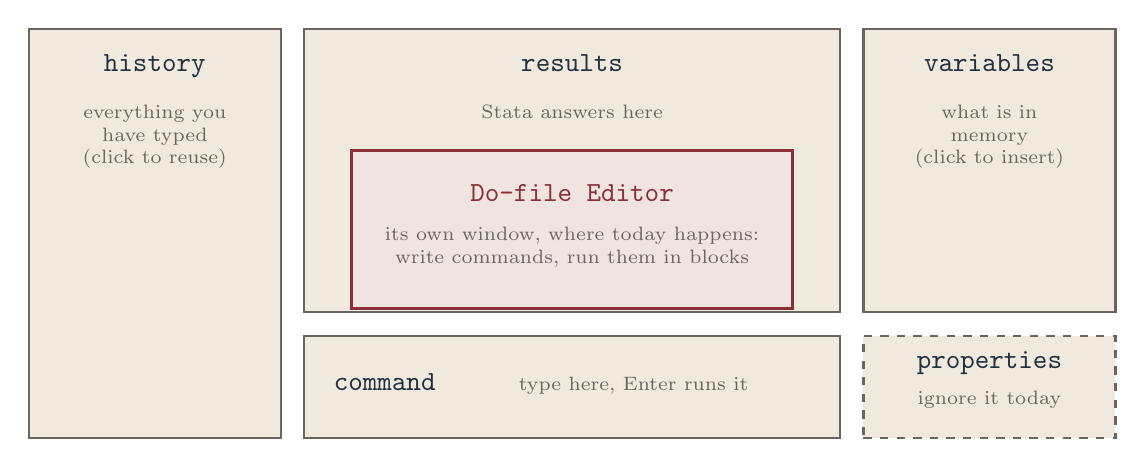
\begin{tikzpicture}
    \node[win, minimum width=3.2cm, minimum height=5.2cm] (rev) at (1.6, 2.6) {};
    \node[winlab, anchor=north] at (1.6, 5.0) {history};
    \node[windesc, anchor=north, text width=2.8cm, align=center] at (1.6, 4.35)
      {everything you\\ have typed\\ (click to reuse)};

    \node[win, minimum width=6.8cm, minimum height=3.6cm] (res) at (6.9, 3.4) {};
    \node[winlab, anchor=north] at (6.9, 5.0) {results};
    \node[windesc, anchor=north] at (6.9, 4.35) {Stata answers here};

    \node[win, minimum width=6.8cm, minimum height=1.3cm] (cmd) at (6.9, 0.65) {};
    \node[winlab, anchor=base west] at (3.75, 0.60) {command};
    \node[windesc, anchor=base west] at (6.1, 0.60) {type here, Enter runs it};

    \node[win, minimum width=3.2cm, minimum height=3.6cm] (var) at (12.2, 3.4) {};
    \node[winlab, anchor=north] at (12.2, 5.0) {variables};
    \node[windesc, anchor=north, text width=2.8cm, align=center] at (12.2, 4.35)
      {what is in\\ memory\\ (click to insert)};

    \node[win, dashed, minimum width=3.2cm, minimum height=1.3cm]
      (prop) at (12.2, 0.65) {};
    \node[winlab, anchor=north] at (12.2, 1.22) {properties};
    \node[windesc, anchor=north] at (12.2, 0.72) {ignore it today};

    % the editor floats IN FRONT of the results pane -- drawn last, on top.
    % It must sit ENTIRELY INSIDE the results pane (x 3.5..10.3, y 1.60..5.20),
    % otherwise its border steps across the pane's border and reads as a bug.
    % center (6.9, 2.65), 5.6 x 2.0 -> spans x 4.1..9.7, y 1.65..3.65
    % clearances: results pane bottom y=1.60 (0.05 inside), pane left x=3.5
    % (0.6), pane right x=10.3 (0.6), "Stata answers here" baseline ~y=4.05
    % (0.40 above), command box top y=1.30 (0.35 below)
    \node[draw=PromptMaroon, very thick, fill=PromptMaroon!10!Paper,
          minimum width=5.6cm, minimum height=2.0cm, align=center]
          (ed) at (6.9, 2.65) {};
    \node[winlab, text=PromptMaroon, anchor=north] at (6.9, 3.35)
      {Do-file Editor};
    \node[windesc, anchor=north, text width=5.4cm, align=center]
      at (6.9, 2.80) {its own window, where today happens:\\
       write commands, run them in blocks};
  \end{tikzpicture}
  \vspace*{0.35cm}

  {\color{WarmGray}\small the four windows are Stata talking to you;
   the editor is you talking back}
\end{frame}

% ===================================================== 6 -- do-file vs log ===
\begin{frame}{You write the do-file; Stata writes the log}
  \centering
  \vspace*{0.9cm}
  % Coordinate map (cm):
  %  dofile : center (1.9, 0),  3.8 x 2.2
  %  stata  : center (6.9, 0),  2.6 x 2.2
  %  log    : center (11.9, 0), 3.8 x 2.2
  %  arrows : (3.8,0)->(5.6,0) label "do" above; (8.2,0)->(10.0,0) label above
  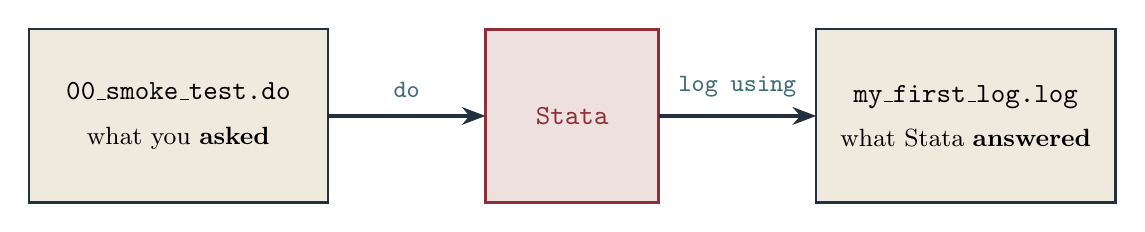
\begin{tikzpicture}
    \node[flowbox] (dofile) at (1.9, 0)
      {{\ttfamily\bfseries 00\_smoke\_test.do}\\[0.4em]
       \small what you \textbf{asked}};
    \node[statabox] (stata) at (6.9, 0)
      {{\ttfamily\bfseries\color{PromptMaroon}Stata}};
    \node[flowbox] (logf) at (11.9, 0)
      {{\ttfamily\bfseries my\_first\_log.log}\\[0.4em]
       \small what Stata \textbf{answered}};
    % Stata box narrowed to 2.2cm so each arrow spans 2.0cm, leaving room for
    % \small mono labels (\scriptsize mono reads ~15% under the size floor)
    \draw[flowarrow] (3.8, 0) -- (5.8, 0)
      node[midway, above, yshift=1mm, font=\ttfamily\small,
           text=SlateTeal] {do};
    \draw[flowarrow] (8.0, 0) -- (10.0, 0)
      node[midway, above, yshift=1mm, font=\ttfamily\small,
           text=SlateTeal] {log using};
  \end{tikzpicture}
  \vspace*{1.1cm}

  {\color{WarmGray}keep both; next week's you can re-read today}
\end{frame}

% ======================================================== 7 -- session map ===
\begin{frame}{Everything you just downloaded}
  \vspace*{0.2cm}
  \begin{center}
  \begin{minipage}{0.97\textwidth}
    \RaggedRight\setlength{\parskip}{0.45em}
    \tagtoday{}{\ttfamily\color{SlateTeal}README.md}
      {\small\color{Ink}--- setup steps + the troubleshooting table}\par
    \tagtoday{}{\ttfamily\color{SlateTeal}code/}
      {\small\color{Ink}--- five do-files (00--04); you run every command
       in them today}\par
    \tagtoday{}{\ttfamily\color{SlateTeal}data/simulated/}
      {\small\color{Ink}--- the dataset; simulated, ships in the ZIP}\par
    \tagown{}{\ttfamily\color{SlateTeal}exercises/}
      {\small\color{Ink}--- three exercises; the first begun together
       in class}\par
    \tagown{}{\ttfamily\color{SlateTeal}extensions/}
      {\small\color{Ink}--- five add-on modules, from loops to project
       structure}\par
    \tagown{}{\ttfamily\color{SlateTeal}docs/}
      {\small\color{Ink}--- the esttab recipe, for your first table}\par
  \end{minipage}
  \end{center}
  \vspace*{0.35cm}
  \centering
  {\color{WarmGray}\small solid tag: hands-on, together, in the next two
   hours.\\ outlined tag: the same style of practice, at your own pace}
\end{frame}

% ======================================================== 8 -- smoke test ====
\begin{frame}{One command tells you whether your setup works}
  \vfill
  \centering
  {\color{WarmGray}\small unzip the download, point Stata at the folder that
   contains {\ttfamily README.md}, then type:}\\[1.1em]
  {\ttfamily\Large\color{Ink}do "code/00\_smoke\_test.do"}\\[1.6em]
  {\ttfamily\large\color{Forest}SMOKE TEST PASSED}\\[0.5em]
  {\color{WarmGray}\small if you see that, sit back. if you see an error,
   read it out loud and we will fix it together}
  \vfill
\end{frame}

% ==================================================== 8 -- divider: look =====
\divider{2}{First, look.}
  {use \, describe \, summarize \, tabulate \, browse\\[0.35em]
   histogram \, scatter \, correlate}{25}

% =================================================== 9 -- divider: clean =====
\divider{3}{Missing is the largest number\\ Stata knows.}
  {count \, list \, replace \, drop\\[0.35em]
   \textcolor{Amber}{if schooling > 12 \& !missing(schooling)}}{20}

% ====================================================== 12 -- the drill =====
% Sits between the break and segment 4. This is the session's one stretch of
% UNGUIDED practice -- the course's usual exercise format in miniature. They have just seen
% the gotcha in segment 3; the break has wiped short-term memory; now they
% must reproduce the !missing() guard unprompted. Exercise 1, task 1.
\begin{frame}{Your turn}
  \vfill
  \centering
  {\Large How many respondents have\\[0.2em]
   \textbf{9 or more years} of schooling?}\\[1.3em]
  {\color{Ink}count it the naive way, then correctly}\\[1.8em]
  {\color{WarmGray}\small three minutes, alone. solutions stay closed.\\
   we compare answers before the next segment}
  \vfill
  \raggedleft
  {\small\color{PromptMaroon}\itshape when your two counts differ, be ready
   to say by how many, and why}
  \par\vspace*{0.3cm}
\end{frame}

% =================================================== 13 -- divider: build ====
\divider{4}{Build the variables the question needs.}
  {generate \, replace \, egen\\[0.35em]
   label variable \, label define \, label values}{15}

% ================================================ 11 -- divider: estimate ====
% The bridge on this divider is shown LIVE at segment 5's open: on the
% cleaned data, -correlate hwage schooling- prints 0.3412 (same units as the
% hook; only the fifteen deleted rows differ) and -correlate lhwage
% schooling- prints 0.3920 (the log step). Each number has one cause.
\divider{5}{Settle the score.}
  {correlate \, regress \, predict\\[0.7em]
   \begin{tabular}{@{}c@{\hspace{0.6em}}c@{\hspace{0.6em}}c@{\hspace{0.6em}}c@{\hspace{0.6em}}c@{}}
   \textcolor{Amber}{-0.0003} & \textcolor{MutedOnInk}{\textrightarrow} &
   \textcolor{Amber}{0.3412} & \textcolor{MutedOnInk}{\textrightarrow} &
   \textcolor{Amber}{0.3920}\\[0.15em]
   {\color{MutedOnInk}\footnotesize raw} & &
   {\color{MutedOnInk}\footnotesize errors deleted} & &
   {\color{MutedOnInk}\footnotesize in logs}
   \end{tabular}}{25}

% ============================================================ 12 -- result ===
\begin{frame}{You just reproduced the OLS benchmark of a real paper}
  \centering
  \vspace*{0.05cm}
  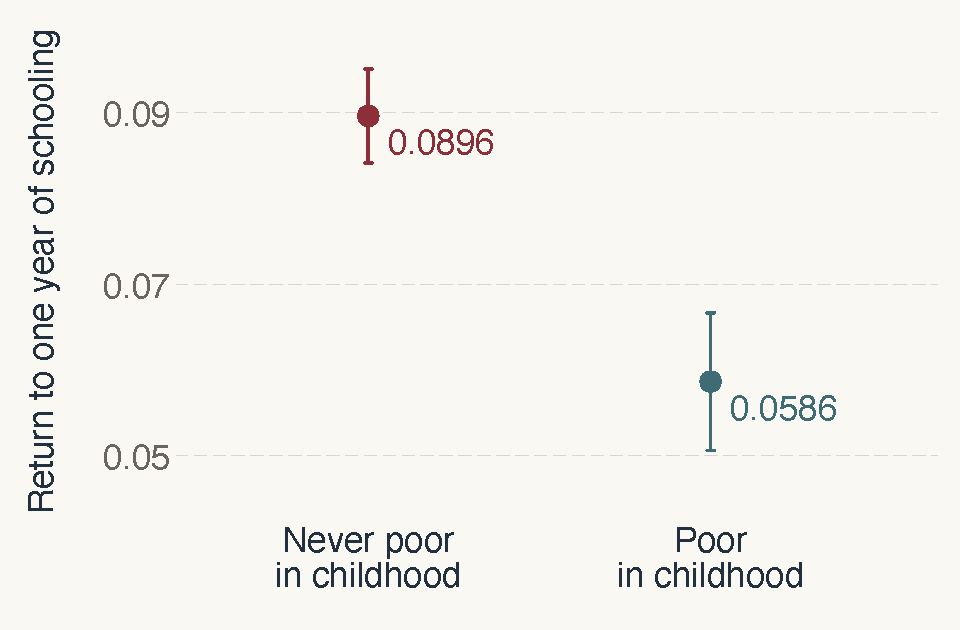
\includegraphics[height=0.58\textheight]{figures/fig_returns_gap}

  \vspace*{0.2cm}
  {\scriptsize\color{WarmGray}Febriady, Post\k{e}pska \& Angelini (2026),
   GLO Discussion Paper 1731.}\\[0.35em]
  {\small\color{WarmGray}OLS, not causal --- schooling is chosen, not
   assigned. {\color{PromptMaroon}\ttfamily extensions/module\_C} shows what
   that hides.}
\end{frame}

% ============================================================= 13 -- repo ====
\begin{frame}{The repo is yours}
  \vfill
  \centering
  {\ttfamily\Large\color{PromptMaroon}github.com/febriady/intro-to-stata}\\[1.1em]
  {\color{Ink}download it again any time; everything re-runs from one fixed
   seed.\\ if your numbers differ, something is wrong, and that is the
   point}\\[1.8em]
  {\small\color{WarmGray}cheat sheets to keep open while you work:}\\[0.3em]
  {\ttfamily\small\color{WarmGray}geocenter.github.io/StataTraining}
  \vfill
\end{frame}

% ========================================================== 14 -- closing ====
{\setbeamercolor{background canvas}{bg=Ink}%
\begin{frame}[plain]
  \centering
  \vfill
  {\ttfamily\bfseries\color{Amber}\Large .\hspace{0.45em}}%
  {\color{white}\LARGE\bfseries Every step was code ---}\\[0.9em]
  {\color{PaperSoft}\Large which means every step can be rerun, checked,
   and improved}\\[0.35em]
  {\color{PaperSoft}\Large by someone who was not in this room.}\\[2.4em]
  {\ttfamily\color{Amber}-0.0003 \textrightarrow\ 0.3920}
  \vfill
\end{frame}}

\end{document}
